\documentclass[12pt]{article}
\usepackage[english]{babel}
\usepackage[utf8x]{inputenc}
\usepackage{amsmath}
\usepackage{graphicx}
\usepackage[colorinlistoftodos]{todonotes}
\usepackage[margin=1in]{geometry}

\begin{document}
	
	\begin{titlepage}
		\newcommand{\HRule}{\noindent\rule{6.5in}{1pt}} % Defines a new command for the horizontal lines, change thickness here
		
		\centering
		
		\textsc{\Large Intro to Artificial Intelligence}\\[.75cm]
		
		\noindent\rule{6.5in}{1.5pt}\\[.75cm]
		{ \huge \bfseries Assignment 1}\\[.4cm]
		{ \large \bfseries Fast Trajectory Planning}\\[.2cm]
		\noindent\rule{6.5in}{1.5pt}\\[1cm]
		
		
		\begin{minipage}{0.4\textwidth}
			\begin{flushleft} \large
				\emph{Authors:}\\
				Brian \textsc{Lin} \\
				Samuel \textsc{Yang}
			\end{flushleft}
		\end{minipage}
		~
		\begin{minipage}{0.4\textwidth}
			\begin{flushright} \large
				\emph{Supervisor:} \\
				Dr.Abdeslam  \textsc{Boularias} % Supervisor's Name
			\end{flushright}
		\end{minipage}\\[2cm]

		
\includegraphics[width=200pt,height=200pt]{RutgersLogo.png}\\[1.5cm]
		\textsc{\Large Rutgers State University of New Jersey}\\[1cm]
		{\large \today}\\[2cm]
		
		\vfill % Fill the rest of the page with whitespace
		
	\end{titlepage}
	
	\twocolumn
	
	\section*{Introduction}
	
	Your introduction goes here! Some examples of commonly used commands and features are listed below, to help you get started.
	
	If you have a question, please use the support box in the bottom right of the screen to get in touch. 
	
	\section*{Part 1 - Understanding the Methods}
	
	\subsection*{A) - East vs North}
		\begin{figure}[!htb]
			\centering
			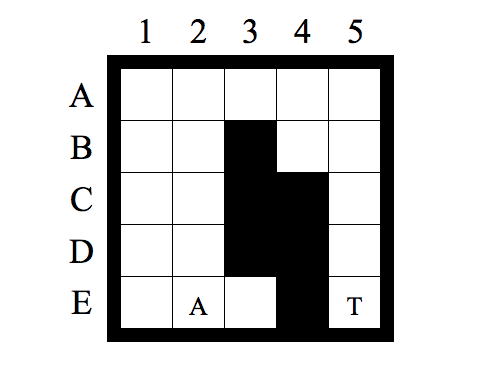
\includegraphics[width=.4\textwidth]{Figure8.png}
			\caption{\label{Figure 8: }Second Example Search Problem}
		\end{figure}
	The agent in the figure above begins it's pathfinding without knowledge of which cells are blocked.  From the perspective of being able to fully observe the maze,
	it appears clear that the best path for the agent is to move north to go around the obstacle.  However, under the initial assumption that all cells are unblocked
	the shortest path from the current cell to the target is to move towards the east, as it has a direct path to the target cell.  Only once the agent has moved to
	the cell to the east, will it observe the blocked cells that do not allow it to use that path and force the agent to find a new path to the target.
	
	\subsection*{B) - Proving Completeness}
	
	\section*{Part 2 - The Effects of Ties}
	
	\section*{Part 3 - Forward vs Backward}
	
	\section*{Part 4 - Proving Heuristics in the Adaptive A*}
	
	\section*{Part 5 - Heuristics in the Adaptive A*}
	
	\section*{Part 6 - Memory Issues}
	
	\iffalse
		\section{Some \LaTeX{} Examples}
		\label{sec:examples}
		
		\subsection{Sections}
		
		Use section and subsection commands to organize your document. \LaTeX{} handles all the formatting and numbering automatically. Use ref and label commands for cross-references.
		
		\subsection{Comments}
		
		Comments can be added to the margins of the document using the \todo{Here's a comment in the margin!} todo command, as shown in the example on the right. You can also add inline comments too:
		
		\todo[inline, color=green!40]{This is an inline comment.}
		
		\subsection{Tables and Figures}
		
		Use the table and tabular commands for basic tables --- see Table~\ref{tab:widgets}, for example. You can upload a figure (JPEG, PNG or PDF) using the files menu. To include it in your document, use the includegraphics command as in the code for Figure~\ref{fig:frog} below.
		
		% Commands to include a figure:
		%\begin{figure}
		%	\centering
			%\includegraphics[width=0.5\textwidth]{frog.jpg}
		%	\caption{\label{fig:frog}This is a figure caption.}
		%\end{figure}
		
		%\begin{table}
		%%	\begin{tabular}{l|r}
				%Item & Quantity \\\hline
				%Widgets & 42 \\
				%Gadgets & 13
		%	\end{tabular}
		%	\caption{\label{tab:widgets}An example table.}
		%\end{table}
		
		\subsection{Mathematics}
		
		\LaTeX{} is great at typesetting mathematics. Let $X_1, X_2, \ldots, X_n$ be a sequence of independent and identically distributed random variables with $\text{E}[X_i] = \mu$ and $\text{Var}[X_i] = \sigma^2 < \infty$, and let
		$$S_n = \frac{X_1 + X_2 + \cdots + X_n}{n}
		= \frac{1}{n}\sum_{i}^{n} X_i$$
		denote their mean. Then as $n$ approaches infinity, the random variables $\sqrt{n}(S_n - \mu)$ converge in distribution to a normal $\mathcal{N}(0, \sigma^2)$.
		
		\subsection{Lists}
		
		You can make lists with automatic numbering \dots
		
		\begin{enumerate}
			\item Like this,
			\item and like this.
		\end{enumerate}
		\dots or bullet points \dots
		\begin{itemize}
			\item Like this,
			\item and like this.
		\end{itemize}
	\fi
	
\end{document}